\documentclass[a4paper, 11pt]{article}
\usepackage[final]{graphicx}
%\usepackage[T1]{fontenc}
\usepackage[utf8]{inputenc}
%\usepackage[margin=2.5cm, nohead]{geometry}
\usepackage{palatino, url, multicol}
\usepackage{amssymb, fancyhdr, latexsym, url, verbatim}
\usepackage{algorithm, algorithmic}
\usepackage{hyperref}
\usepackage[all]{xy}
%\usepackage{listings}
\usepackage[english]{babel}
\usepackage[format=plain,labelfont=bf,up,textfont=it,up]{caption}
\usepackage{xspace}
%\usepackage{subfigure} % has to be loaded after caption to prevent clash Commented, because subfig is the newer (and presumably
% better) version of subfigure...
%\usepackage{subfig}
\usepackage{subcaption}
\usepackage{xcolor}
\usepackage[all]{xy}
% For awesome graphs:
\usepackage{tikz}
\usetikzlibrary{shapes.geometric}

%\usepackage[titles,subfigure]{tocloft}
%\setlength{\cftbeforesecskip}{0.1cm}

\newcommand{\todo}[1]{\colorbox{red}{\color{white}#1}}

\begin{document}

%\vspace*{1cm}


\begin{center}
\Huge \textbf{Bomberman: An Evaluation of Two Types of AI}\\
\vspace*{0.8cm}
\Large John Aivalis () \& Maarten Inja (5872464) \& \\ Tobias Tahl? () \& Maarten de Waard (5894883) 

\vspace*{4cm}

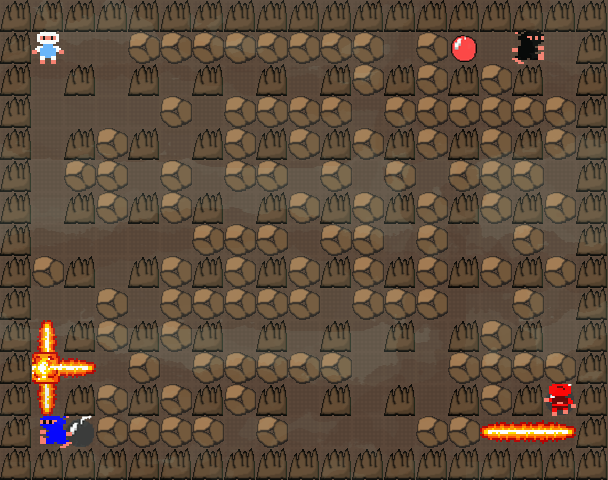
\includegraphics[width=10cm]{resources/bbman}

\vfill
\today

\end{center}
\thispagestyle{empty}

\newpage

\newpage
\pagenumbering{roman}
\vspace*{-2cm}
\tableofcontents

\newpage

\begin{abstract}
We have created two types of artificial intelligent agents for the game
Bomberman. Both types of agents employ a different strategy to destroy
its opponents; one seeks out its enemies as soon as possible while the other
one attempts to find as many power ups as possible. In this document we will
show how the artificial intelligence behind these agents works and that it
is better to go in for the kill as soon as possible, rather than to upgrade
first.
\end{abstract}

\pagenumbering{arabic}
\section{Introduction}
%\begin{document} 
For this project we chose to implement two types of artificial intelligent agents for the game Bomberman.

%\subsection{A Brief Introduction}
The game Bomberman (also known as Dynablaster) is a strategic, maze-based, 2D
video game franchise originally developed by Hudson Soft. It was originally
published in 1983 and until now over 80 games have featured
Bomberman\cite{bomberman2013}.
The goal of the game is to complete levels by strategically placing bombs in order to eliminate enemy players and demolish obstacles. 
Bombs are the only weapon at the players disposal and are a key aspect of the
game. The bombs will explode a brief amount of time after they have been placed
and will kill any player that is within their reach and demolish up to one
obstacle in each of the four directions they affect. 

Power ups are an essential part in Bomberman as they increase the reach of the
fire of the bombs, the speed of the player or how many bombs one player can have
placed on the map at the same time. One can imagine that these power ups are
advantageous as they allow the player to gain more powers, speed to or from the enemy and surround enemies entirely with bombs.

To investigate the effect of power ups we have crafted two artificial intelligent agents which both employ different strategies in regards to upgrades. One AI employs a strategy to get to and kill an enemy player as fast as possible, we shall call this AI `Kill-First-AI'. The second AI first attempts to gain as much upgrades as possible before engaging the other players, we shall call this AI `Upgrade-First-AI'.


%\section{Related Work}
%\label{sec:relatedWork}
%\input{sections/relatedWork}

\section{Approach}
%\subsection{ Our project setup}
For this project we made use of an already existing implementation of the game platform in Java\footnote{The source for the existing implementation: \url{https://code.google.com/p/javabomber/}}. This game was mostly multiplayer oriented, it did have an AI implementation which was however, too simplistic.
Initially we made some alterations to the given project in order to organize the source code in a way that makes more sense. Some of the steps we took in favor of refactoring the code were the following:
\begin{itemize}
\item Pulled up a `Map' class. This enabled us to organize the path finding algorithms we used in robust fashion.
\item Created a `GenericAI' abstract class containing important methods and variables. Here are the methods that are used by all AI implementations. This class is extended by any AI implementation we made.
\item Created a `Cell' class  representative of a cell of the Map.
\end{itemize}
In order to create, test and benchmark the different AI's, a great amount of alterations were done
to the game's menu and the underlying main class. Eventually two AI classes were
created, respectively called the `SimpleAI' class for the Kill-First-AI, and the
`MapClearAI' for the Upgrade-First-AI.




\section{Implementation}
\label{sec:implementation}
\subsection{Kill-First-AI}
We thought of various ways to implement AI agents for the game. Our final AI implementation is based on the decision tree model. The logic behind the implementation is illustrated in Figure \ref{fig:tree1}.

\tikzset{
    every node/.style={
        font=\scriptsize
    },
    decision/.style={
        shape=rectangle,
        minimum height=1cm,
        text width=2cm,
        text centered,
        rounded corners=1ex,
        draw,
        label={[yshift=0.125cm]left:yes},
        label={[yshift=0.125cm]right:no},
    },
    outcome/.style={
        shape=ellipse,
        fill=gray!15,
        draw,
        text width=1.5cm,
        text centered
    },
    decision tree/.style={
        edge from parent path={[-latex] (\tikzparentnode) -| (\tikzchildnode)},
        %sibling distance=5cm,
        level distance=2cm
    }
}
\tikzset{level 1/.style={sibling distance=6cm}}
\tikzset{level 2/.style={sibling distance=3cm}}

\begin{figure}
\centering
%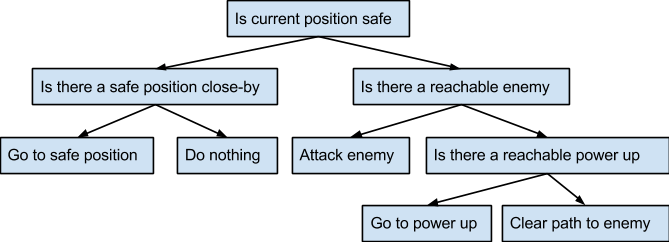
\includegraphics[width=10cm]{resources/tree1}
\begin{tikzpicture}[node distance =0cm, auto]
\node [decision] {Is current position safe?}
    [decision tree]
    child { node [decision] { Is there a reachable enemy? } 
        child { node [outcome] { attack enemy } }
        child { node [decision] { Is there a reachable powerup? } 
            child { node [outcome] { Go to powerup } }
            child { node [outcome] { Clear path to enemy } }
        }
    }
    child { node [decision] { Is there a safe position nearby?}
            child { node [outcome] { Go to safe position} }
            child { node [outcome] { Do nothing} }
    };
\end{tikzpicture}
\caption{Decision Tree for the Kill-First AI}
\label{fig:tree1}
\end{figure}

As you can see the logic behind the AI agents is relatively simple, in a step by step breakdown of the figure above we see the states of the agent being divided into two different categories. One is the case in which the current position of the agent is safe and the agent has time to plot it’s  next move and the other is when the agents position is threatened by a bomb. This is the major concern of the agent when checking for the next move. 
In case the current position is threatened by a close-by bomb or the player is located on a bomb (in our implementation of the game this can only occur after it itself has placed it), the player looks for a way to avoid the threat by moving away from the bomb. If looking for a safe position returns no viable results then there is nothing to do and the player loses. If not the player will follow the path returned to him by the ‘findClosestSafeSpot()’ method.
On the other subtree we see the tactics the bot will make use of in order to achieve his goal in defeating his opponents. The ‘isEnemyReachable()’ function will return whether if the closest opponent to the player is within reach, meaning if there is no obstacle in the path returned using the A* algorithm. If there is at least one obstacle in that path then the bot assumes that there is still time to pick up power-ups instead and focuses on that. Furthermore the instant the enemy becomes reachable, the bot’s top priority becomes attacking the opponent instead.


\subsubsection{Attacking Tactics}
Attacking the enemy can be achieved in various ways. Initially our tactic was the following: if the player has an opponent within 3 blocks away from him then he would place a bomb in order to attack him. Later on during the evaluation process we thought that we could introduce the concept of the bot already knowing the firepower it has in it’s disposal. That is how we came up with the final simple approach which was the following: if the bot has a player within reach (with respect to the bot’s firepower) then it will place a bomb to attack them.

Moving and Path Finding Tactics
Pulling up the Map class had a lot of positive impact in making the moving of the players easier. This enabled us to make use of all the functions necessary to implement path finding algorithms. The path finding algorithm we made use of was the A* algorithm. At this point we had to determine the costs of moving through the various types of blocks in the map. We have three types of map cells in the map those are the following :
\begin{itemize}
\item Empty spaces
\item Obstacles
\item Walls
\end{itemize}

Obviously the empty spaces and walls have trivial scores of 1 and undefined (infinity) respectively. However, the one that took some effort in order to figure out, was the obstacle cost.
Initially the players will have obstacles between them and still would require to calculate the distances between them. The final cost we assigned to the ‘obstacle’ class of map cell finally was 4. We observed some weird behaviours when this score was 3. That is the bots would end up trapped by their bombs after placing them. We assumed that the difference between 3 and 4 is that when the cost is fixed to 4 the bot prefer moving around an obstacle more to blasting through it. That is the reason why it will never try to reach a safe position after placing a bomb by blasting it’s way through another obstacle.

\subsection{Upgrade-First-AI}
\begin{figure}
\centering
%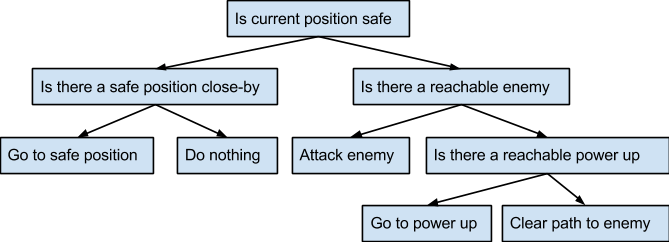
\includegraphics[width=10cm]{resources/tree1}
\begin{tikzpicture}[node distance =0cm, auto]
\node [decision] {Is current position safe?}
    [decision tree]
    child { node [decision] { Is there a reachable powerup? } 
        child { node [outcome] { Go to powerup } }
        child { node [decision] { Are more powerups needed? } 
            child { node [outcome] { Blow up nearest reachable block} }
            child { node [decision] { Is an enemy reachable? } 
                child { node [outcome] { Attack enemy } }
                child { node [outcome] { Do nothing } }
            }
        }
    }
    child { node [decision] { Is there a safe position nearby?}
            child { node [outcome] { Go to safe position} }
            child { node [outcome] { Do nothing} }
    };
\end{tikzpicture}
\caption{Decision Tree for the Upgrade-first AI}
\label{fig:treeUpgradeFirst}
\end{figure}
As can be seen in figure \ref{treeUpgradeFirst}, this AI has an extension on the
Kill-First's decision tree. This one aims to get at least 3 bombs and a
firepower of 4 squares in all directions, before trying to kill the opposing
forces.



\todo{Explain this AI here}


%\section{Method}
%\label{sec:method}
%\input{sections/method}

\section{Results}
\begin{table}
\centering
\begin{tabular}{l|l}
\textbf{AI Name} & \textbf{Number of wins}\\\hline
\textit{Kill-First-AI} & 48 \\
\textit{Upgrade-First-AI} & 27\\
\end{tabular}
\caption{Results of 100 matches between the Kill-First-AI and the
Upgrade-First-AI. The rest of the results are draws, meaning that the game did
not end within 10,000 time steps (which should equal slightly more than
2 minutes of play time if one were to play the games oneself)}
\label{tab:results}
\end{table}

In order to compare the AI's with each other, a simple benchmark tool was
created. This tool runs a number of matches and keeps the results of these
matches. After the competition is done, the number of victories per bot type is
printed. Table \ref{tab:results} shows the results of a benchmark running 100
games.

\subsection{Analysis}
When looking at the results, it can be concluded that the Kill-First-AI works
better than the Upgrade-First-AI. To find a reason for this result, we can look
at the individual games of the one versus the other.

The main cause of losing for the Upgrade-First-AI seems to be that most of the
times, the enemy has already reached it, before it is done `upgrading'. The
collecting behavior of the bot seems to work a lot worse, when the enemy is
constantly threatening him with bombs. In many situations the Upgrade-First-AI
gets himself into trouble by still placing bombs in his neighbourhood, while the
enemy tries to kill him. This results in the bot having too many bombs in its
surroundings to escape from, resulting in a lost game. 

In most games where the
Upgrade-First bot does get enough time to get all the power ups required, it beats the
opponent.




\section{Discussion}
Can we now honestly advocate one type of strategy over another? Obviously, no.

\todo{Discuss the following stuff in more detail.}

\begin{itemize}
\item Things might be different with different upgrades, which other versions of Bomberman clearly do have.
\item Overall path finding might benefit one AI more than the other
\item Tweaks in low level behaviour might favor one type of AI
\item `Normal' Bomberman works differently in regards to collision detection
\item Different kind of maps might require different kind of strategies
\end{itemize}


\section{Future Work}
%\begin{document}
There is more future work we could do in order to evaluate different
strategies for AI in Bomberman.

As mentioned in the discussion the game we worked with still differs
from original Bomberman games, we could reduce this difference by
implementing some of the following game features:
\begin{itemize}
\item Implement more kind of upgrades
\item Implement other maps
%\item Fix collision detection
\end{itemize}

There are also more research questions remaining:
\begin{itemize}
\item We could implement and evaluate different kind of strategies. For example
a mix of the strategies we implemented could work even better
(focus on collecting upgrades until a foe appears, then focus on the foe). Or
collect a certain amount of upgrades of each kind before going after the opponent
could be even better.
\item Try and see what strategies would work the best for more than two
players. One can image free for all play, or team play with any kind of number
of players. It is yet unknown what kind of strategy would suffice in such
situations.
\end{itemize}


\newpage
\bibliographystyle{plain}
\bibliography{references}

\newpage
\pagenumbering{alph}
\section{Appendix}
\input{sections/appendix}

\end{document}





